\documentclass[a4paper, 12pt, french]{article}
\usepackage[utf8]{inputenc}
\usepackage[T1]{fontenc}
\usepackage{babel}

%Images
\usepackage{graphicx} 
\graphicspath{{src/dev/}}

%Code
\usepackage{listings}
\usepackage{color}

\definecolor{dkgreen}{rgb}{0,0.6,0}
\definecolor{gray}{rgb}{0.5,0.5,0.5}
\definecolor{mauve}{rgb}{0.58,0,0.82}

\lstset{frame=tb,
  language=Java,
  aboveskip=5mm,
  belowskip=5mm,
  framesep=3mm,
  showstringspaces=false,
  columns=flexible,
  basicstyle={\small\ttfamily},
  numbers=none,
  numberstyle=\tiny\color{gray},
  keywordstyle=\color{blue},
  commentstyle=\color{dkgreen},
  stringstyle=\color{mauve},
  breaklines=true,
  breakatwhitespace=true,
  tabsize=3
}

%Commandes perso
\newcommand{\hr}{\noindent\rule{13.7cm}{0.4pt}}

%Metas
\title{Java OO}
\author{Elanis - https://github.com/Elanis/LaTeX-cheatsheets}

\begin{document}
	\maketitle

	\section{Programme par defaut}

	\begin{lstlisting}
	public class Hello {
		public static void main(String[] args) {
			System.out.println("Hello World !!!");
		}
	}
	\end{lstlisting}

	\section{Programmation orientée objet}
	\subsection{Bases}

	\begin{lstlisting}
	public class Hello {
		private int x;

		// Constructeur
		public Hello(int x) {
			this.x = x;
		}

		// Encapsulation: getter/setter
		public int getX() { return x; }
		public void setX(x) { this.x = x; }
	}
	\end{lstlisting}

	Portées disponibles:
	\begin{description}
		\item[Privé:] Mot clé \emph{private}, inaccessible hors de l'objet
		\item[Protégé:] Mot clé \emph{protected}, inaccessible hors de la hiérarchie des classes
		\item[Friendly:] \emph{Aucun mot clé}, inaccessible en dehors du package.
		\item[Public:] Mot clé \emph{public}, totalement accessible
	\end{description}

	\begin{lstlisting}
	public class Hello {
		private int x;

		// Constructeur par recopie
		public Hello(hellOther) {
			this.x = hellOther.x;
		}
	}
	\end{lstlisting}

	\begin{lstlisting}
	public class Personne {
		// Attribut statique (dependant de la classe et non de l'objet)
		private static int NB_TOTAL = 0;

		private int id;

		public Hello() {
			this.id = ++NB_TOTAL;
		}

		// Methode statique
		public static int getNbPersonne() {
			return NB_TOTAL;
		}
	}
	\end{lstlisting}

	\subsection{Heritage}

	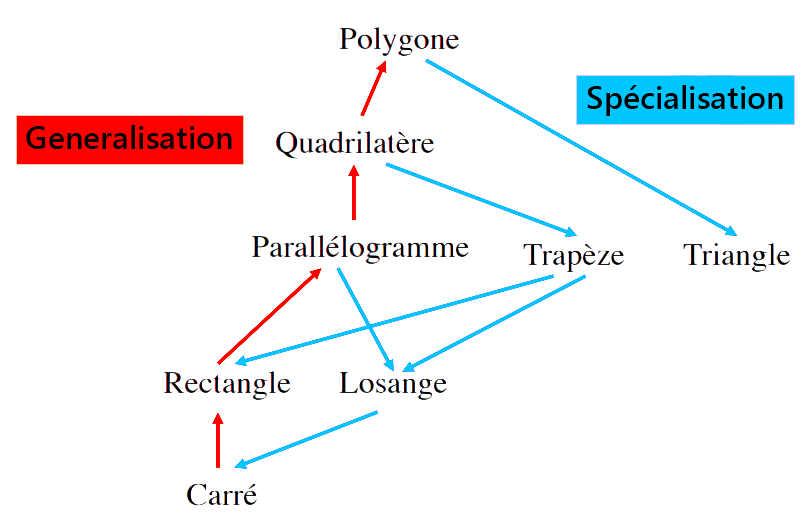
\includegraphics[width=13.8cm]{java_00_heritage}

	\begin{lstlisting}
	public class Parent {
		// ...

		public final int variable; // final = ne peut pas etre redefini dans les enfants
	}

	public class Enfant extends Parent {
		// ...
		public Enfant() {
			super(); // appelle la meme fonction du parent (ici le constructeur)
		}
	}

	public class Descendant extends Enfant {
		// ...
	}
	\end{lstlisting}
\end{document}